The FESTIM code was compared to TMAP7 \sidecite{longhurst_tmap7_2008}.
Since TMAP7 is a 1D code, a 1D test case was created.
% maybe say a bit more on TMAP7 here


\subsubsection{Geometry}
The 1D simulation case is a \SI{8.5}{mm}-thick composite slab made of W, Cu and CuCrZr (see Figure \ref{fig: monoblock 1D geometry}).
The plasma facing surface $\Gamma_\mathrm{top}$ is located at $x=\SI{0}{mm}$ and the surface cooled by water $\Gamma_\mathrm{coolant}$ is located at $x=\SI{8.5}{mm}$.

\begin{figure}
    \begin{overpic}[width=0.75\linewidth]{Figures/Chapter3/monoblocks/interface_condition/iter case/Monoblock 1D.pdf}
        \put(40, 50){\SI{6}{mm}}
        \put(40, 8){W}
        \put(62, 50){\SI{1}{mm}}
        \put(65, 8){Cu}
        \put(72, 50){\SI{1.5}{mm}}
        \put(72, 8){CuCrZr}
        \put(6, 25){\large$\Gamma_\mathrm{top}$}
        \put(85, 25){\large$\Gamma_\mathrm{coolant}$}
    \end{overpic}
     \caption{2D ITER monoblock geometry showing W armour \cruleme[grey]{0.3cm}{0.3cm}, Cu interlayer \cruleme[orange]{0.3cm}{0.3cm}, CuCrZr alloy cooling pipe  \cruleme[yellow]{0.3cm}{0.3cm}}
     \label{fig: monoblock 1D geometry}
\end{figure}

\subsubsection{Boundary Conditions}
The boundary conditions are detailed in Equation \ref{eq: code comparison BCs}.

\begin{subequations}
    \begin{align}
    T &= \SI{1200}{K}\quad \text { on } \Gamma_\mathrm{top}\\
    c_\mathrm{m} &=  \frac{\varphi_\mathrm{imp} \cdot R_p}{D} \quad \text { on } \Gamma_\mathrm{top}\\
    T &= \SI{373}{K} \quad \text { on } \Gamma_\mathrm{coolant}\\
    -D \nabla c_\mathrm{m} \cdot \vec{n} &= K_\mathrm{CuCrZr} \cdot c_\mathrm{m}^{2} \quad \text { on } \Gamma_\mathrm{coolant}  
    \end{align}
    \label{eq: code comparison BCs}
\end{subequations}
with $\varphi_\mathrm{imp} = \SI{5e23}{m^{-2}.s^{-1}}$ the implanted particle flux, $R_p = \SI{1.25}{nm}$ the implantation depth, $\vec{n}$ the normal vector and $K_\mathrm{CuCrZr} = 2.9 \times 10^{-14}\cdot \exp{(-1.92/(k_B\cdot T))}$ the recombination coefficient of the CuCrZr (in vacuum) expressed in \si{m^4.s^{-1}} \sidecite{anderl_deuterium_1999}.

The Dirichlet boundary condition on $\Gamma_\mathrm{top}$ for the hydrogen transport corresponds to a flux balance between the implanted flux and the flux that is retro-desorbed at the surface (see Section \ref{triangle model}).

\subsubsection{Results}

\begin{figure*} [h]
    \centering
    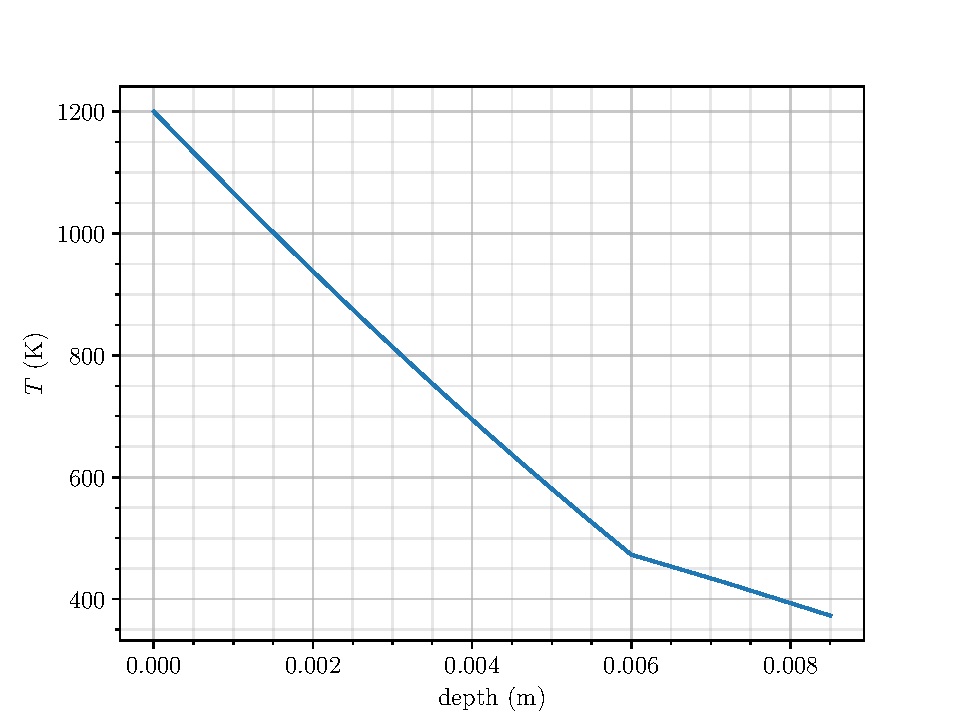
\includegraphics[width=0.5\linewidth]{Figures/Chapter3/monoblocks/interface_condition/iter case/temperature_1D.pdf}
    \caption{ITER monoblock temperature simulated by FESTIM (1D and 2D).}
    \label{fig: temperature}
\end{figure*}

\begin{figure} [h]
    \centering
    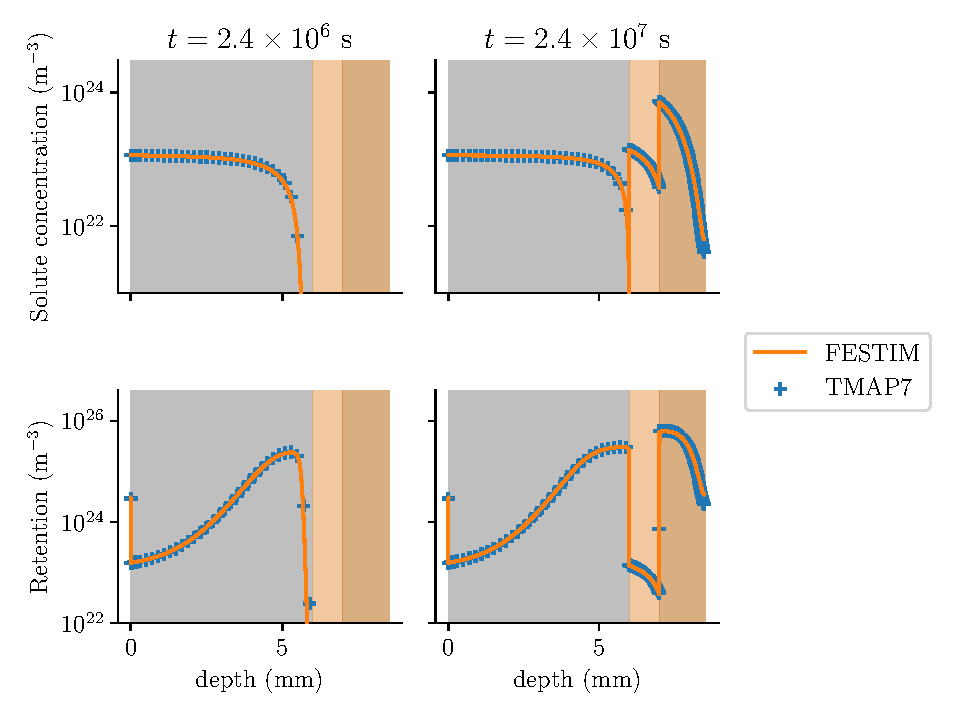
\includegraphics[width=\linewidth]{Figures/Chapter3/monoblocks/interface_condition/iter case/comparison_codes.pdf}
    \caption{Comparison of results provided by FESTIM, TMAP7 and ABAQUS}
    \label{fig: code comparison}
\end{figure}

A comparison test was made with the code TMAP7 with this set of parameters and very good agreement was found between the two codes (see Figure \ref{fig: code comparison}).
